\documentclass[spanish, fleqn]{article}
\usepackage{babel}
\usepackage[utf8]{inputenc}
\usepackage{amsmath}
\usepackage{amsfonts}
\usepackage{mathrsfs}
\usepackage{dcolumn}
\usepackage[colorlinks, urlcolor=blue]{hyperref}
\usepackage{fourier}
\usepackage{tikz}
\usepackage{float}
\usetikzlibrary{arrows,shapes,snakes,automata,backgrounds,petri,babel,positioning}
\usepackage{pgf}
\usepackage[top = 2.5cm, bottom = 2cm, left = 2cm, right = 2cm]{geometry}
\definecolor{navyblue}{RGB}{0,148,222}
\definecolor{supercolor}{RGB}{0,148,12}
\tikzstyle{transition}=[rectangle,thick,draw=black!75,fill=black!20,minimum size=8mm]

\newcommand{\num}{1}

\title{ILI-255: Informática Teórica \\[0.4\baselineskip]
       Tarea \#\num \\
       \emph{``"It’s not my fault”''}
      }
\author{\href{mailto:daniel.quinteros.12@sansano.usm.cl}{Roberto Fuentes}\\
201173037-2}
\date{10 de Abril 2017}

\begin{document}
\maketitle

\thispagestyle{empty}

\section*{Desarrollo}
    
    \begin{enumerate}
    
    \item Pregunta 1:
        \begin{enumerate}
        \item Nos piden una expresión regular que permita identificar un $RUT$ válido en el formato de chileno. Para esto,  Luego, definiremos el alfabeto "$\alpha$" para denotar los \textcolor{red}{numeros de un digito} (0,1,2,\ldots,9) y definiremos el alfabeto $\beta$ para denotar los \textcolor{blue}{numeros de un digito sin el 0} (1,2,\ldots,9). Un $RUT$ debe terminar con "- ($\alpha\mid$k)". Sabiendo esto, un rut puede tener el siguiente formato: $número$ - ($número \mid$ k), $número$ $numero$ - ($número \mid $k), $número$ $numero$ $numero$ - ($número \mid$ k) y finalmente cualquiera de estas 3 opciones seguido de $(.$ $número$ $numero$ $numero$) seguido de ($número \mid$ k). Una expresión regular para el $RUT$ chileno seria entonces:
        
         $$\textbf{\textit{RE}}: (\beta\mid\beta\alpha\mid\beta\alpha\alpha) (.\alpha\alpha\alpha)^* - (\alpha\mid\text{k}) $$
        
        \item Un DFA que puede representar esta expresión regular es la siguiente:
        
        	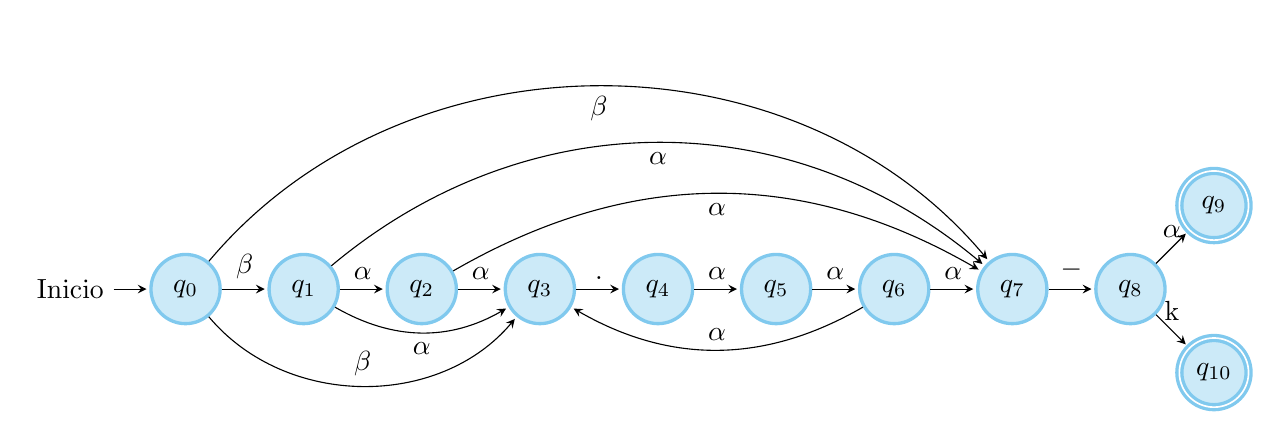
\begin{tikzpicture}[shorten >=1pt,node distance=1.5cm,on grid, >=stealth, initial text=Inicio, every state/.style={draw=navyblue!50,very thick,fill=navyblue!20}, bend angle=35]]
        		\node[state,initial]    (q_0)                          {$q_0$};
                \node[state,]	(q_1) [right of = q_0]         {$q_1$};
                \node[state]            (q_2) [right of = q_1]         {$q_2$};
                \node[state]            (q_3) [right of = q_2]         {$q_3$};
                \node[state]            (q_4) [right of = q_3]         {$q_4$};
                \node[state]            (q_5) [right of = q_4]         {$q_5$};
                \node[state]            (q_6) [right of = q_5]         {$q_6$};
                \node[state]            (q_7) [right of = q_6]         {$q_7$};
                \node[state]            (q_8) [right of = q_7]         {$q_8$};
                \node[state,accepting]            (q_9) [above right of = q_8]         {$q_9$};
                \node[state,accepting]            (q_10) [below right of = q_8]         {$q_{10}$};
                
            \path[->]   (q_0) edge node [above]                 {\(\beta\)} (q_1)
                        (q_1) edge node [above]                 {\(\alpha\)} (q_2)
                        (q_2) edge node [above]                 {\(\alpha\)} (q_3)
                        (q_3) edge node [above]                 {$.$} (q_4)
                        (q_4) edge node [above]                 {\(\alpha\)} (q_5)
                        (q_5) edge node [above]                 {\(\alpha\)} (q_6)
                        (q_6) edge node [above]                 {\(\alpha\)} (q_7)
                        (q_7) edge node [above]                 {$-$} (q_8)
                        (q_8) edge node [above]                 {\(\alpha\)} (q_9)
                        (q_8) edge node [above]                 {k} (q_10)
                        (q_0) edge[bend left=50] node [below]   {\(\beta\)} (q_7)
                        (q_1) edge[bend left=40] node [below]   {\(\alpha\)} (q_7)
                        (q_2) edge[bend left=30] node [below]   {\(\alpha\)} (q_7)
                        (q_6) edge[bend left=30] node [above]   {\(\alpha\)} (q_3)
                        (q_0) edge[bend right=50]node [above]   {\(\beta\)} (q_3)
                        (q_1) edge[bend right=30]node [below]   {\(\alpha\)} (q_3);
        	\end{tikzpicture}      
        
        
        
        \end{enumerate}    
        
        \item Pregunta 2: \\
        \\
        Aplicando el algoritmo $\epsilon$ - closure a nuestro NFA nos queda lo siguiente:
        
   \begin{flalign*}
       &\epsilon-closure\text{ }\{ a\}=\{a\} \\
       &0: a,b,c,d,e \\
       &1: e,d \\ 
       &A = \{a\} \\
       &B = \{a,b,c,d,e\} \\
       &C = \{d,e\}&&
   \end{flalign*}
  B: 
    \begin{flalign*}
       &\epsilon-closure\text{ }\{ a,b,c,d,e\}=\{a,b,c,d,e\}\\
       &0: a,b,c,d,e \\
       &1: b,d,e \\ 
       &D = \{b,e,d\} &&
   \end{flalign*}
   C:
   \begin{flalign*}
       &\epsilon-closure\text{ }\{ d,e\}=\{d,e\}\\
       &0: e \\
       &1: \emptyset \\ 
       &e = \{b,e,d\} &&
   \end{flalign*}
   D:   
   \begin{flalign*}
       &\epsilon-closure\text{ }\{ b,e,d\}=\{b,e,d\}\\
       &0: c,e \\
       &1: e \\ 
       &G = \{c,e\}&&
   \end{flalign*}
   E:
   \begin{flalign*}
       &\epsilon-closure\text{ }\{e\}=\{e\}\\
       &0: \emptyset \\
       &1: \emptyset &&
   \end{flalign*}
   F
   \begin{flalign*}
       &\epsilon-closure\text{ }\{\emptyset\}=\{\emptyset\}&&
   \end{flalign*}
   G:
   \begin{flalign*}
       &\epsilon-closure\text{ }\{c,e\}=\{c,e\}\\
       &0: \emptyset \\
       &1: b \\
       &H: \{b\}&&
   \end{flalign*}
   H:
   \begin{flalign*}
       &\epsilon-closure\text{ }\{b\}=\{b\}\\
       &0: c \\
       &1: e \\
       &I: \{c\}&&
   \end{flalign*}
   I:
   \begin{flalign*}
       &\epsilon-closure\text{ }\{c\}=\{c\}\\
       &0:\emptyset \\
       &1: b \\
       &H: \{b\}&&
   \end{flalign*}
        
Luego construimos la tabla de transiciones:

\begin{center}

\begin{tabular}{ | m{1cm} | m{5cm} | m{1cm} | m{1cm} | } 
\hline
\textbf{DFA} & \textbf{NFA} & \textbf{0} & \textbf{1} \\ 
\hline
A & \{a\} & B & C \\
\hline
B & \{a,b,c,d,e\} & B & D \\
\hline
C & \{d,e\} & E & F \\ 
\hline
D & \{d,e,b\}& G & E \\ 
\hline
E & \{e\} & F & F \\ 
\hline
F & \{$\emptyset$\} & F & F \\ 
\hline
G & \{e,c\} & F & H \\ 
\hline
H & \{b\} & I & E \\ 
\hline
I &  \{c\} & F & H \\ 
\hline
\end{tabular}
\end{center}

Finalmente el DFA nos queda de la siguiente forma:
\begin{center}

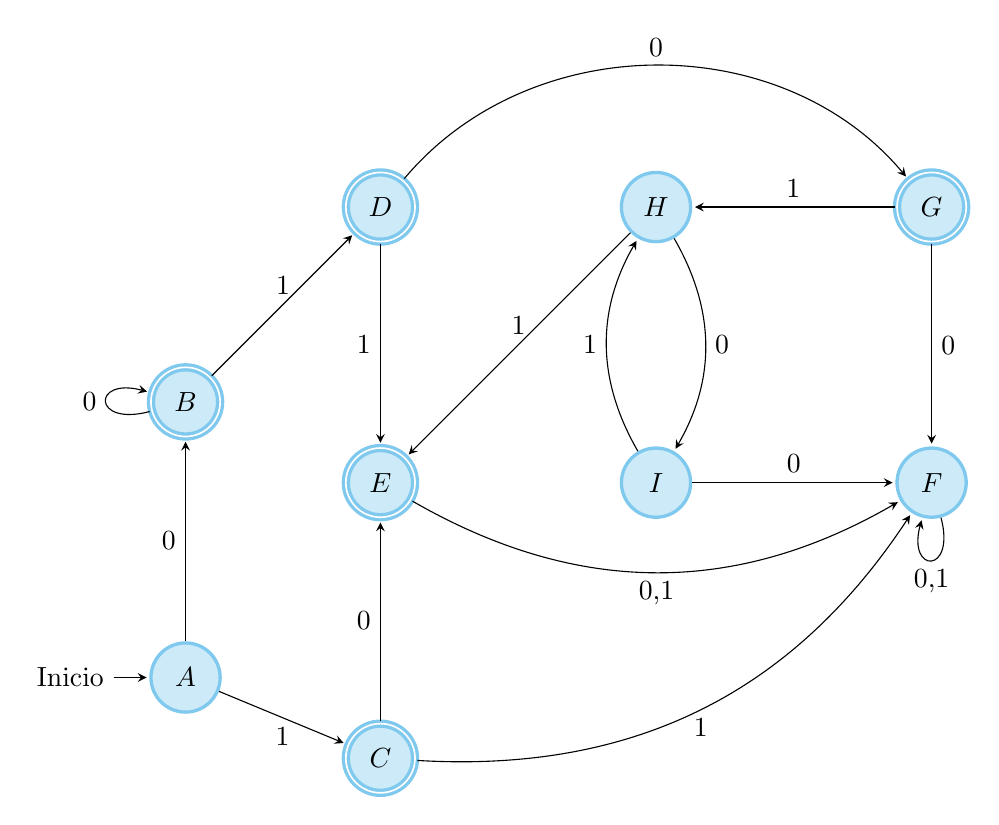
\begin{tikzpicture}[shorten >=1pt,node distance=3.5cm,on grid, >=stealth, initial text=Inicio, every state/.style={draw=navyblue!50,very thick,fill=navyblue!20}, bend angle=35]]
        		\node[state,initial]    (a)                        {$A$};
                \node[state,accepting]	(b) [above of = a]         {$B$};
                \node[state,accepting]  (d) [above right of = b]   {$D$};
                \node[state,accepting]  (e) [below of = d]         {$E$};
                \node[state,accepting]  (c) [below of = e]         {$C$};
                \node[state]            (h) [right of = d]         {$H$};
                \node[state]            (i) [right of = e]         {$I$};
                \node[state,accepting]  (g) [right of = h]         {$G$};
                \node[state]            (f) [right of = i]         {$F$};
                
                
                \path[->]   
                        (a) edge node [left]                  {0}   (b)
                        (a) edge node [below]                 {1}   (c)
                        (b) edge node [above]                 {1}   (d)
                        (d) edge node [left]                  {1}   (e)
                        (c) edge node [left]                  {0}   (e)
                        (c) edge[bend right=30] node [below]  {1}   (f)
                        (d) edge[bend left=50] node [above]   {0}   (g)
                        (e) edge[bend right=30] node [below]  {0,1} (f)
                        (g) edge node [right]                 {0}   (f)
                        (g) edge node [above]                 {1}   (h)
                        (h) edge node [above]                 {1}   (e)
                        (i) edge node [above]                 {0}   (f)
                        (h) edge[bend left=30] node [right]   {0}   (i)
                        (i) edge[bend left=30] node [left]    {1}   (h)
                        (b) edge [loop left]   node [left]    {0}   (b)
                        (f) edge [loop below]  node [below]   {0,1} (f);
                        
        	\end{tikzpicture}      
\end{center}    


\item Pregunta 3: \\
\\
Primero creamos un automata cuyo $output$ sean números divisibles por 3. El automata nos queda de la siguiente forma:

        	\begin{center}
        	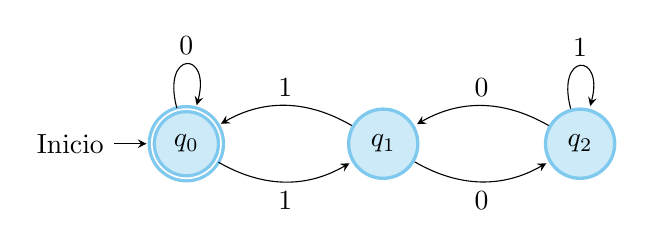
\begin{tikzpicture}[shorten >=1pt,node distance=2.5cm,on grid, >=stealth, initial text=Inicio, every state/.style={draw=navyblue!50,very thick,fill=navyblue!20}, bend angle=35]]
        		\node[state,initial,accepting]    (q_0)                  {$q_0$};
                \node[state]	                  (q_1) [right of = q_0] {$q_1$};
                \node[state]                      (q_2) [right of = q_1] {$q_2$};
                
            \path[->]   (q_0) edge[bend right=30]  node [below]   {\(1\)} (q_1)
                        (q_1) edge[bend right =30] node [above]   {\(1\)} (q_0)
                        (q_1) edge[bend right=30]  node [below]   {\(0\)} (q_2)
                        (q_2) edge[bend right =30] node [above]   {\(0\)} (q_1)
                        (q_0) edge[loop above]     node [above]   {0}     (q_0)
                        (q_2) edge[loop above]     node [above]   {1}     (q_2);
        	\end{tikzpicture} 
            \end{center}
Este grafo nace de lo siguiente:

Consideramos que un numero puede ser escrito de la siguiente forma: $num = 3*a + b$, donde b es el resto. Queremos que cada numero que acepte el automata tenga b = 0, por lo que armamos tres estados $q_1$,$q_2$ y $q_3$, siendo estos los restos 0,1,2. Analizamos entonces los arcos:

\begin{enumerate}

\item Al empezar en el estado $q_0$ y leer un 0, nos quedamos en el estado $a_0$, y el numero 0 es divisible por 3.

\item Estando en el estado $q_0$ y leyendo un 1, nos vamos al estado $q_1$. Esto lo hacemos ya que el número que se forma (1) en decimal nos da un resto de 1.

\item Cuando estamos en el estado $q_1$ y leemos un 0, nos movemos al 2. Esto ocurre ya que el número en binario generado (10) en decimal nos da un resto de 2.

\item Cuando estamos en el estado $q_1$ y leemos un 1, nos vamos al estado $q_0$. Esto ocurre ya que el binario que nos entrega el automara (11) en decimal nos da un resto de 0.

\item Cuando estamos en el estado $q_2$ y leemos un 0, nos vamos al estado $q_1$. Esto ocurre ya que el binario generado (100) en decimal nos entrega un resto de 1

\item Cuando estamos en el estado $q_2$ y leemos un 1, nos quedamos en el estado 2. Esto ocurre porque el binario generado (101) en decimal nos entrega un resto de 2

\end{enumerate}

Por lo que la tabla de transiciones debe ser la siguiente:

\begin{center}

\begin{tabular}{ | m{2cm} | m{1cm} | m{1cm} | } 
\hline
Estado & 0 & 1 \\
\hline
$q_0$ & 0 & 1\\
\hline
$q_1$ & 2 & 0 \\ 
\hline
$q_2$  & 1 & 2 \\ 
\hline
\end{tabular}
\end{center}

Quedando el grafo resultante que se propuso anteriormente. El problema que tenemos con este DFA es que no incluye la condicion de que la cantidad de 0's y 1's sea par, ya que tanto en el nodo $q_0$ como el nodo $q_1$ se pueden repetir una cantidad impar de 0's y 1's. Para esto, tomemos el caso de $q_0$. Cambiamos la condicion de repetir muchas veces el 0, yendo con un 0 a otro estado $q_3$ y devolviendonos al mismo estado $q_0$. Asi, nos aseguramos de que la cantidad de 0 siempre sea multiplo de 2 (es decir par), y realizamos lo mismo con el nodo $q_2$. Haciendo esto nos queda:

        	\begin{center}
        	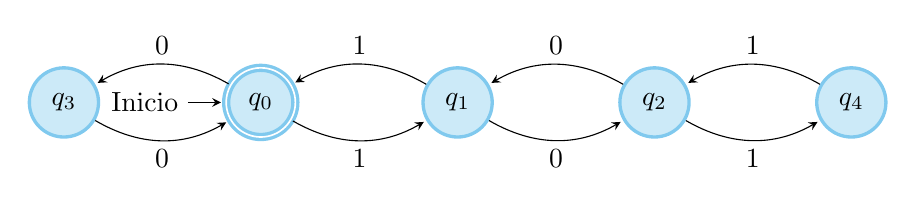
\begin{tikzpicture}[shorten >=1pt,node distance=2.5cm,on grid, >=stealth, initial text=Inicio, every state/.style={draw=navyblue!50,very thick,fill=navyblue!20}, bend angle=35]]
        		\node[state,initial,accepting]    (q_0)                  {$q_0$};
                \node[state]	                  (q_1) [right of = q_0] {$q_1$};
                \node[state]                      (q_2) [right of = q_1] {$q_2$};
                \node[state]                      (q_3) [left of =  q_0] {$q_3$};
                \node[state]                      (q_4) [right of = q_2] {$q_4$};
                
            \path[->]   (q_0) edge[bend right=30]  node [below]   {\(1\)} (q_1)
                        (q_1) edge[bend right =30] node [above]   {\(1\)} (q_0)
                        (q_1) edge[bend right=30]  node [below]   {\(0\)} (q_2)
                        (q_2) edge[bend right =30] node [above]   {\(0\)} (q_1)
                        (q_0) edge[bend right=30]  node [above]   {\(0\)} (q_3)
                        (q_3) edge[bend right =30] node [below]   {\(0\)} (q_0)
                        (q_2) edge[bend right=30]  node [below]   {\(1\)} (q_4)
                        (q_4) edge[bend right =30] node [above]   {\(1\)} (q_2);
        	\end{tikzpicture} 
            \end{center}
\end{enumerate}
\end{document}